\documentclass[a4paper,UTF8]{paper}
\usepackage{ctex}
\usepackage{amsmath}
\usepackage{pdfpages}
\usepackage{graphicx}
\usepackage{wrapfig}
\usepackage{listings}
\usepackage{multicol}
\usepackage{color}
\usepackage{alltt}
\usepackage{marvosym}
% Style definition file generated by highlight 3.6, http://www.andre-simon.de/ 

% Highlighting theme: Print 

\newcommand{\hlstd}[1]{\textcolor[rgb]{0,0,0}{#1}}
\newcommand{\hlnum}[1]{\textcolor[rgb]{0,0,0}{#1}}
\newcommand{\hlesc}[1]{\textcolor[rgb]{0,0,0}{#1}}
\newcommand{\hlstr}[1]{\textcolor[rgb]{0,0,0}{#1}}
\newcommand{\hlpps}[1]{\textcolor[rgb]{0,0,0}{#1}}
\newcommand{\hlslc}[1]{\textcolor[rgb]{0.4,0.4,0.4}{\it{#1}}}
\newcommand{\hlcom}[1]{\textcolor[rgb]{0.4,0.4,0.4}{\it{#1}}}
\newcommand{\hlppc}[1]{\textcolor[rgb]{0,0,0}{\bf{#1}}}
\newcommand{\hlopt}[1]{\textcolor[rgb]{0,0,0}{\bf{#1}}}
\newcommand{\hllin}[1]{\textcolor[rgb]{0.53,0.53,0.53}{#1}}
\newcommand{\hlkwa}[1]{\textcolor[rgb]{0,0,0}{\bf{#1}}}
\newcommand{\hlkwb}[1]{\textcolor[rgb]{0,0,0}{\bf{#1}}}
\newcommand{\hlkwc}[1]{\textcolor[rgb]{0,0,0}{\bf{#1}}}
\newcommand{\hlkwd}[1]{\textcolor[rgb]{0,0,0}{\bf{#1}}}
\definecolor{bgcolor}{rgb}{1,1,1}


\newcommand{\tabincell}[2]{\begin{tabular}{@{}#1@{}}#2\end{tabular}}
\begin{document}
\tableofcontents
\clearpage
\section{程序架构}
我们采用C++/Qt来开发现行平台,平台的核心是一个Traffic\_v1对象,如图\ref{UML}所示。

\begin{figure}
\centering
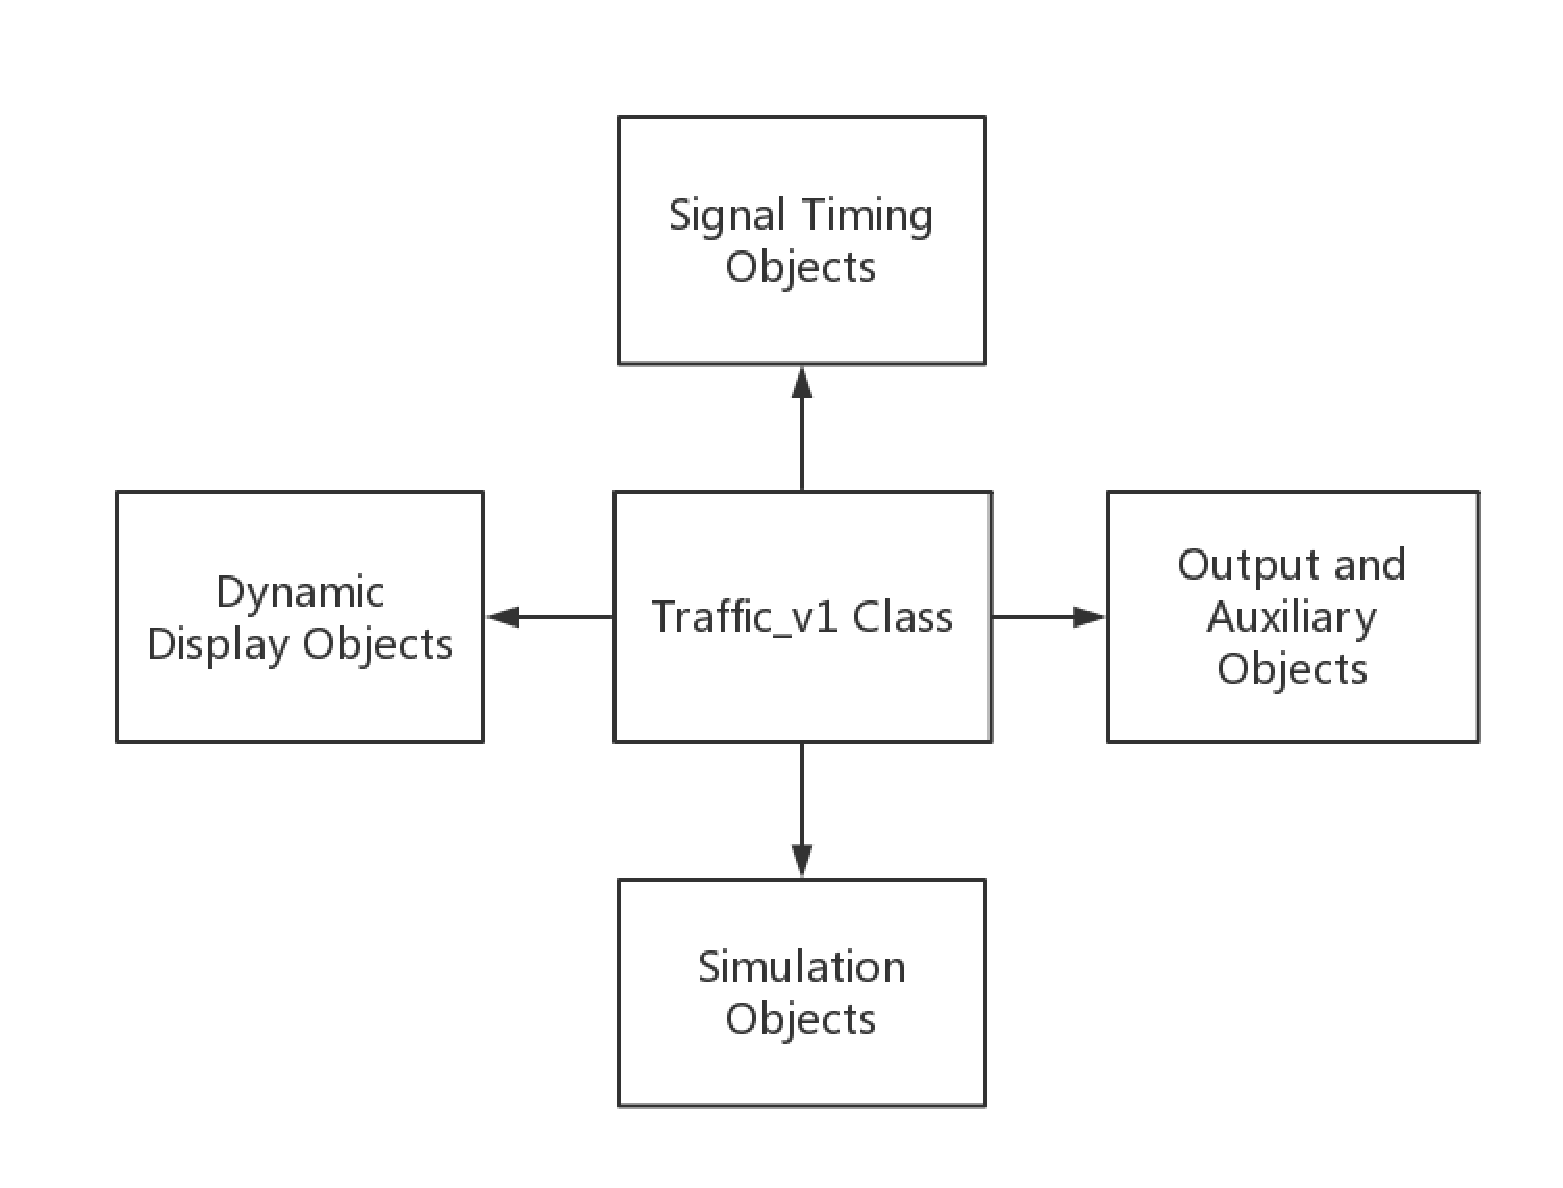
\includegraphics[width=\textwidth]{Diagram.eps}
\caption{Traffic\_v1 类的架构}
\label{UML}
\end{figure}

\subsection{显示模块}
这些模块用来动态显示仿真过程和控制仿真执行的流程,如设置仿真速度等。主要包括按键,标签,滑动条等对象。

当仿真每向前执行一步的时候,平台将刷新仿真模块来显示仿真过程中的具体情况,整个函数将完成如下几个步骤。

\begin{enumerate}
\item 绘制交通路口的基本要素

根据信号配时模块给出的信号相位,显示模块将绘制红绿灯。同时,显示模块将绘制交通路口前的车道,目前设定绘制30m长,22.5m宽的车道

\item 绘制车辆

绘制模块将绘制即将进入路口的车辆和驶离路口的车辆,在所有的车辆中,即将驶入路口的车辆是接受控制的,而驶离路口的车辆是不接受控制的,平台将为他们补全整个的控制策略。

\item 绘制交通路口中的车辆轨迹线

平台不处理车辆在交通路口内的行为,因此采用绘制车辆在路口中的轨迹线来表示车辆可能存在的位置。当车辆驶入交通路口时,我们假设左转车辆在交通路口的滞留时间是3s,而执行车辆在交通路口内的滞留时间是2s,右转车辆在交通路口内的滞留时间是1s,这些参数可以通过平台代码中的参数简单的修改。在滞留时间内的车辆会在交通路口内显示一道轨迹线,表示车辆可能在的位置。

可以看出,轨迹线的交点多少可以表示交通路口的混乱程度,如果交通路口内存在着大量的轨迹线交点,交通效率将受到影响,同时交通危险性将显著提升。而这一部分应当是信号配时的主要工作。
\end{enumerate}

\subsection{仿真模块}
这是整个平台的核心模块,通过设置的仿真速度,平台给出一个间隔为1ms(高速模式),10ms(中速模式),100ms(低速模式),1000ms(调试模式)的信号。

当触发信号被接受时,平台将按照如图\ref{int}所示的行为进行相关的操作。

\begin{figure}
\centering
\includegraphics[width=\textwidth]{TimeFlow.png}
\caption{平台执行流程}
\label{int}
\end{figure}

在执行过程中,进程控制模块根据用户设定的停止条件决定是否终止仿真,之后,每个道路的入口将根据车辆生成算法来生成新的车辆。之后,用户策略将根据车辆类型的不同分别和用户选择的模式应用在不同的车辆上。同时系统策略负责离开交通路口的车辆的行为和诸如进入交通路口等边界情况的处理。

所有的策略均调整车辆的加速度,在运动学仿真模块,平台将通过车辆现有的位置,速度和加速度计算车辆下一时刻的位置和速度。

最后,平台将处理进入交通路口的车辆和即将离开研究路段的车辆的边界情况。

程序之后完成界面的重绘工作,并等待下一个触发信号的到来。

根据现行平台实现,在一般配置的笔记本电脑上,在10ms的仿真时钟间隔的情况(中速模式)下系统压力还是比较合适的,同时平台产生的仿真数据也是比较合理的。当仿真时钟间隔被调整到1ms(高速模式),在交通压力过大的情况下会出现时序问题。

\subsection{输出和辅助模块}
这部分模块的主要作用是在系统重绘时或一些特殊情况发生时输出仿真结果。

随着仿真的进行,系统在可执行文件所在目录根目录中建立文件夹"result",在此文件夹内建立包含4张CSV表,一个子文件夹,这个子文件夹的命名规则是

\centerline{\textbf{'日期+时间+仿真模式选择'}}

四张CSV表中保存记录了不同类型的数据。

\begin{enumerate}
\item car.csv

这张表保存记录了车辆的初始速度(init\_velocity),理论到达时间(thoritical\_time) 和实际到达时间(act\_time), 理论到达时间被定义为车辆以最大加速度加速到最大速度之后进行匀速直线运动到达路口所花的时间。 理论到达时间 thoritical\_time 和实际到达时间 act\_time之间的差异可以描述车辆经过这段区域所浪费的时间。

\item stop.csv

这张表保存记录了每个车道上车辆的总停车次数和总共路口车辆的停车次数以及停车次数占整个车辆数量的比例。

\item road.csv

这张表记录了每个时刻驶离某一车道的车辆数量和离开系统的车辆数量,和相对应的平均值,这张表往往被用来检查仿真的合理性。

\item stop\_time.csv

这张表记录了每个车道上的总共的停车时间和整个系统内的通车时间以及分担到每个车辆上的停车时间。
\end{enumerate}

总的来说,road.csv 被用来观察 仿真过程是否正常执行而其他三个表用来评价整个所采用的驾驶策略的效率

另外,停车行为由车辆速度低于某个阈值决定,同时,当车辆停下时,停车时间不断累加,而停车次数不发生变化。这一点在长期停车时尤其明显。

\subsection{信号配时模块}

信号配时模块满足了用户自主设置信号周期和相位的要求,三个按键'set red behind'、 'set green behind'、 'set yellow behind' 被用来设置黑色时间线之后的信号相位。

同时,这个界面可以用来调整信号的周期。因此,通过调整黑色时间线或指定确定的调整时间,不断重复设置时间线之后的信号相位等工作,用户可以完全自主的完成信号的配时工作。

同时,左侧的界面将显示当前交通路口车辆的轨迹线,当前时间是黑色轨迹线所指示的时间。通过交通轨迹线的显示和对交叉情况的判断,系统可以在一定程度上辅助用户完成更好更合理的交通信号配时工作。
\subsection{平台界面}

仿真模块的界面和信号配时的界面如图\ref{cap1} 和图\ref{cap2}所示。

\begin{figure}
\centering
\includegraphics[width=\textwidth]{cap1.jpg}
\caption{仿真模块界面}
\label{cap1}
\includegraphics[width=\textwidth]{cap2.jpg}
\caption{信号配时模块的界面}
\label{cap2}
\end{figure} 

在仿真模块界面上点击'Edit Traffic Light'按钮可以激活信号配时模块的界面,如果用户关闭信号配时模块界面,他所作的变更将被保存同时仿真模块界面将被再次激活。

\clearpage
\section{算法简介}
\subsection{基础假设和参数}
首先,我们认为对车辆而言,车辆的加速度是可控的物理量,同时,其他的物理量(如速度和位置)由车辆的加速度和当前时刻的速度根据如下运动学公式确定: 
$$v(t+\Delta_t)=v(t)+a\Delta_t$$
$$x(t+\Delta_t)=x(t)+v(t)\Delta_t+0.5a\Delta_t^2$$ 

另外,由于车辆的加速度也不能被准确的控制,我们在策略给出加速度的准确值之后加入了一个正态分布的随机噪声,尤其是后文提到的人工驾驶的车辆模型,引入的正态分布随机噪声更大。

同时,平台对车辆的加速度和速度也有着限制,我们认为车辆加速度的绝对值的最大值是$a_{max}$,被用来限制车辆的加速过程和刹车过程。另外,车辆的最大速度被限制为$v_{max}$,车辆的最低速度被限制为$v_{min}$。

不论选择了那种驾驶策略,如果策略给出的加速度值大于最大加速度$a_{max}$或者小于$-a_{max}$,抑或是计算得到的速度大于最大速度或小于最小速度,程序将自动将这些值设定为对应的边界值。如果车辆受到红灯影响而被迫刹车停车,最小速度限制将被设定为0来描述可能的停车行为。但不论如何,倒车行为是永远不可接受的。

同时我们假设车辆期望的速度,$v_{exp}$,被设定为车辆最高限速的80\%。

为了简化模型,我们认为在所研究路段进行驾驶的过程中,车辆不进行变道行为。这个假设在现实情况中也是可以被接受的,因为受到交通法规和规则的限制,车辆在交通路口前的变道行为往往是被禁止或限制的。车辆需要在进入交通路口之前完成相关的变道工作,因此我们的假设是合理的,同时仅仅从交通效率的角度来看,换道行为也只能降低交通效率,不利于对驾驶策略进行评估。因此,因为平台的评估主要以策略为主,就不考虑车辆的换道行为了。

因此,在一个车道进行驾驶的车辆可以被描述成一个队列结构,即$Q_{in}$。

\subsection{车辆产生算法}
我们假设车辆的到达过程是一个泊松过程,这个到达过程受到下面算法的限制。

我们假设泊松过程的强度是$\lambda$到达车辆而定时间间隔$S_n,S_{n-1}$可以被表述为 
$$P((S_n-S_{n-1}\le t) = 1 - e^{-\lambda t}$$
因为仿真过程的时间间隔被设定为0.1s,每小时的平均车流量即为$$\bar{F}=36000\lambda$$

对于一个方向的车辆,车辆的小时流量被仿真界面上的交通流控制滑块设定之后,这个方向的车流量将按照特定的泊松过程进行生成$\lambda=\displaystyle{\frac{\bar{F}}{3600}}$, 并且被压入每个方向上的等待队列$Q_{pending}$。

在生成车辆之后,下一步是考虑车辆应当放入那个车道,我们认为车辆放入合理车道的可能性是相同的,合理车道被定义为车辆放入之后仍能安全行驶的车道。其具体定义可以被定义为,车辆生成位置($S_{start}$)和最后一个车辆的距离$X_{-1}$之间的距离大于安全行驶距离$S_{safe}$即,$$X_{-1}-S_{start}\le S_{safe}$$

遍历所有符合条件的合理车道,并且将$Q_{pending}$中的车辆等可能的放入其中的一条车道上。新生成的车辆的位置为$S_{start}$,即车辆生成线的位置。

如果目前没有合适的放入车辆的车道,车辆将被保留在$Q_{pending}$队列中并等待下一个仿真循环。

车辆生成的算法在整个仿真流程的第二步进行,紧随仿真流程控制模块。
\subsection{路口车辆排队的产生和消散}
\label{section:feq}
为了描述路口车辆排队的产生和消散过程,我们对每个驶入交通路口的车道引入队列$Q_{block}$。同时,根据现行信号相位和队列的长度,我们采用的所有控制策略几乎均采用如下提到的简单算法
\begin{enumerate}
\item 红灯

如果队列$Q_{in}$中的第一辆车辆和队列$Q_{block}$中的最后一辆车辆之间的距离小于控制距离$S_{control}$,队列$Q_{in}$中的第一个车辆将刹车并期望停在队列$Q_{block}$最后一辆车的期望距离之后。这个两车之间的期望距离被定义为$S_{stop}$,用来描述在队列$Q_{block}$中的车辆间距。 

如果$Q_{block}$为空并且$Q_{in}$中的第一辆车辆和停车线之间的距离小于$S_{control}$,$Q_{in}$中的头车以停车线$S_{end}$为目标进行刹车。

如果$Q_{in}$中的头车距离路口太远以至于上述两条均不满足,$Q_{in}$中的头车将自由驾驶。

同时,$Q_{block}$中的车辆应当停车等待直到信号灯变绿。
\item 绿灯
在车辆驾驶策略的设计中,队列$Q_{in}$的第一辆车辆和队列$Q_{block}$中的最后一个车辆(如果他存在)之间的距离不应当小于安全距离$S_{safe}$。 如果两车之间距离小于安全距离,后车将采取刹车行为。
\end{enumerate}
综上所示,整个算法的简明思路可以用如下的伪代码表述\\ 

\noindent
\ttfamily
\hlstd{}\hllin{01\ }\hlkwa{if\ }\hlstd{}\hlopt{(}\hlstd{Q\textunderscore block}\hlopt{.}\hlstd{}\hlkwd{empty}\hlstd{}\hlopt{())\{}\\
\hllin{02\ }\hlstd{\ }\hlkwa{if\ }\hlstd{}\hlopt{(}\hlstd{Light\ }\hlopt{==\ }\hlstd{Green}\hlopt{)}\\
\hllin{03\ }\hlstd{}\hlstd{\ \ }\hlstd{Q\textunderscore in}\hlopt{.}\hlstd{}\hlkwd{first}\hlstd{}\hlopt{().}\hlstd{}\hlkwd{drive\textunderscore freely}\hlstd{}\hlopt{();}\\
\hllin{04\ }\hlstd{\ }\hlkwa{else}\\
\hllin{05\ }\hlstd{}\hlstd{\ \ }\hlstd{Q\textunderscore in}\hlopt{.}\hlstd{}\hlkwd{first}\hlstd{}\hlopt{().}\hlstd{}\hlkwd{brake\textunderscore to}\hlstd{}\hlopt{(}\hlstd{S\textunderscore end}\hlopt{);}\\
\hllin{06\ }\hlstd{}\hlopt{\}}\\
\hllin{07\ }\hlstd{}\hlkwa{else}\hlstd{}\hlopt{\{}\\
\hllin{08\ }\hlstd{\ }\hlkwa{if}\hlstd{}\hlopt{(}\hlstd{Q\textunderscore block}\hlopt{.}\hlstd{}\hlkwd{last}\hlstd{}\hlopt{().}\hlstd{pos}\hlopt{{-}}\hlstd{Q\textunderscore in}\hlopt{.}\hlstd{}\hlkwd{first}\hlstd{}\hlopt{().}\hlstd{pos}\hlopt{$<$\ }\hlstd{S\textunderscore control}\hlopt{)}\\
\hllin{09\ }\hlstd{}\hlstd{\ \ }\hlstd{Q\textunderscore in}\hlopt{.}\hlstd{}\hlkwd{first}\hlstd{}\hlopt{().}\hlstd{brake\textunderscore to\\
\hllin{10\ }}\hlstd{\ \ }\hlstd{}\hlopt{(}\hlstd{Q\textunderscore block}\hlopt{.}\hlstd{}\hlkwd{last}\hlstd{}\hlopt{().}\hlstd{pos}\hlopt{{-}}\hlstd{S\textunderscore stop}\hlopt{);\ }\\
\hllin{11\ }\hlstd{\ }\hlkwa{else}\\
\hllin{12\ }\hlstd{}\hlstd{\ \ }\hlstd{Q\textunderscore in}\hlopt{.}\hlstd{}\hlkwd{first}\hlstd{}\hlopt{().}\hlstd{}\hlkwd{drive\textunderscore freely}\hlstd{}\hlopt{();}\\
\hllin{13\ }\hlstd{}\hlopt{\}}\hlstd{}\\
\mbox{}
\normalfont
\normalsize


代码中brake\_to(desired\_pos) 函数的意义是设置车辆的加速度使得车辆能够刹车到期望的位置上

另外,队列$Q_{block}$的产生和消散将遵循如下的模型。

\begin{enumerate}
\item 产生/增长

当队列$Q_{in}$中的第一辆车辆距离距离$Q_{block}$中的最后一辆车辆(如果不存在,则设为停车线$S_{end}$)的距离小于停车距离$S_{stop}$时,这辆车将从$Q_{in}$中移除并被加入到$Q_{block}$中。

\item 消散

当信号灯为绿灯时,队列$Q_{block}$中的所有车辆将按照消散速度$v_{dis}$向前移动,由于这个速度值设定得很小,使得加速过程和其他的相关过程可以忽略笔记。当车辆越过停车线时,将被从队列$Q_{block}$中移除。

\end{enumerate}

以上所述均可以用下面的伪代码表示

\noindent
\ttfamily
\hlstd{}\hllin{01\ }\hlkwa{if\ }\hlstd{}\hlopt{(}\hlstd{light\ }\hlopt{==\ }\hlstd{green}\hlopt{)\{}\\
\hllin{02\ }\hlstd{\ Q\textunderscore block}\hlopt{.}\hlstd{}\hlkwd{all\textunderscore move\textunderscore forward}\hlstd{}\hlopt{(}\hlstd{v\textunderscore dis}\hlopt{)}\\
\hllin{03\ }\hlstd{}\hlopt{\}}\\
\hllin{04\ }\hlstd{}\hlkwa{else}\hlstd{}\hlopt{\{}\\
\hllin{05\ }\hlstd{\ }\hlkwa{if}\hlstd{}\hlopt{(!}\hlstd{Q\textunderscore block}\hlopt{.}\hlstd{}\hlkwd{empty}\hlstd{}\hlopt{())\{}\\
\hllin{06\ }\hlstd{}\hlstd{\ \ }\hlstd{}\hlkwa{if}\hlstd{}\hlopt{(}\hlstd{Q\textunderscore block}\hlopt{.}\hlstd{}\hlkwd{last}\hlstd{}\hlopt{().}\hlstd{pos}\hlopt{{-}}\hlstd{Q\textunderscore in}\hlopt{.}\hlstd{}\hlkwd{first}\hlstd{}\hlopt{().}\hlstd{pos\\
\hllin{07\ }}\hlstd{\ \ \ }\hlstd{}\hlopt{$<$\ }\hlstd{S\textunderscore stop}\hlopt{)\{}\\
\hllin{08\ }\hlstd{}\hlstd{\ \ \ }\hlstd{Vehicle\ v}\hlopt{;}\\
\hllin{09\ }\hlstd{}\hlstd{\ \ \ }\hlstd{v}\hlopt{=}\hlstd{Q\textunderscore in}\hlopt{.}\hlstd{}\hlkwd{getfirst}\hlstd{}\hlopt{();}\\
\hllin{10\ }\hlstd{}\hlstd{\ \ \ }\hlstd{Q\textunderscore block}\hlopt{.}\hlstd{}\hlkwd{push}\hlstd{}\hlopt{(}\hlstd{v}\hlopt{);}\\
\hllin{11\ }\hlstd{}\hlstd{\ \ }\hlstd{}\hlopt{\}}\\
\hllin{12\ }\hlstd{\ }\hlopt{\}}\\
\hllin{13\ }\hlstd{\ }\hlkwa{else}\hlstd{}\hlopt{\{}\\
\hllin{14\ }\hlstd{}\hlstd{\ \ }\hlstd{}\hlkwa{if}\hlstd{}\hlopt{(}\hlstd{S\textunderscore end}\hlopt{{-}}\hlstd{Q\textunderscore in}\hlopt{.}\hlstd{}\hlkwd{first}\hlstd{}\hlopt{().}\hlstd{pos}\hlopt{$<$\ }\hlstd{S\textunderscore stop}\hlopt{)\{}\\
\hllin{15\ }\hlstd{}\hlstd{\ \ \ }\hlstd{Vehicle\ v}\hlopt{;}\\
\hllin{16\ }\hlstd{}\hlstd{\ \ \ }\hlstd{v}\hlopt{=}\hlstd{Q\textunderscore in}\hlopt{.}\hlstd{}\hlkwd{getfirst}\hlstd{}\hlopt{();}\\
\hllin{17\ }\hlstd{}\hlstd{\ \ \ }\hlstd{Q\textunderscore block}\hlopt{.}\hlstd{}\hlkwd{push}\hlstd{}\hlopt{(}\hlstd{v}\hlopt{);}\\
\hllin{18\ }\hlstd{}\hlstd{\ \ }\hlstd{}\hlopt{\}}\\
\hllin{19\ }\hlstd{\ }\hlopt{\}}\\
\hllin{20\ }\hlstd{\ }\\
\hllin{21\ }\hlopt{\}}\hlstd{}\\
\mbox{}
\normalfont
\normalsize


以上描述了路口队列的产生和消散过程和这个模型和其他道路要素的联动。经过仿真实验,由于模型设定的假设导致的差别是可以忽略的。由于这个模型的引入,我们可以简单的将车辆的驾驶和排队模型解耦,使得我们能够更简单的实现其他的驾驶模型。

\section{驾驶模型概述}
\subsection{基本模型}

在对人工驾驶模型和自主驾驶模型进行描述的过程中,车辆的跟驰模型和自由驾驶模型是经常被使用的模型。因此在讨论其他的驾驶模型和控制策略之前,我们首先讨论这两个模型

\subsubsection{自由驾驶模型的实现}

在不存在速度引导的情况下,车辆的行为可以大体上被分类为自由驾驶模型和人工驾驶模型两类,这两个模型将在本节和下一节讨论。控制距离$S_{control}$被定义成前后两个车辆之间的距离。因此,上述两种驾驶模型将按照如下的规则进行选择。

\begin{enumerate}
\item 当和前车之间的距离小于预先设定的控制距离$S_{control}$时,我们选择跟驰模型描述车辆的行为

\item 当和前车之间的距离大于控制距离$S_{control}$时,我们选择自由驾驶模型来描述车辆的行为。自由驾驶模型中,车辆将通过一些加速度的调整来将自己的速度设定为期望速度$v_{exp}$,如果当前的速度值和$v_{exp}$相近,车辆所采取的加速度可能比较小,如果当前速度和$v_{exp}$相差比较远,车辆所采取的加速度可能比较大,这描述了车辆在出现可能的停车之后的起步加速直至正常行驶的过程。

同样,由于有随机噪声的存在,如果车辆的速度大于最大速度$v_{max}$,车辆将采取适当的制动步骤。
\end{enumerate}

\subsubsection{车辆跟驰模型的实现}
\label{cf}
上文已经提到,当和前车的距离过近的时,车辆将采用跟驰模型来描述其行为,在我们使用的策略中,我们采用了Wiedemann生理——心理模型来描述车辆的行为,即:
$$a_n(t+\Delta_t)=\frac{[\Delta v_{n,n-1}(t)]^2}{2[\Delta x_{n,n-1}(t)-S_{exp}]}+a_{n-1}(t)$$

在上面的式子中,$S_{exp}$代表了期望的车辆之前的安全行驶距离,因为车辆在是将交通路口时速度变化十分剧烈,因此期望距离$S_{exp}$不应是一个常数。因此,根据交通安全法规和驾驶一般情况,我们使用了和前车速度线性相关的跟驰距离来描述期望的跟驰距离,因此,期望跟驰距离$S_{exp}$如下所示:
$$S_n(t)=\alpha v_{n-1}(t)+S_{safe}$$
其中$S_{safe}$和\ref{section:feq}提到的相同,而常数$\alpha$可根据实际情况和经验设定。

一旦车辆之间的间距小于$S_{exp}$,亦即车辆之间的距离过近,车辆将采取紧急刹车制动,车辆采取的加速度值可能根据具体情形的不同而变化,在大多数情形下,车辆将采取的刹车加速度绝对值为$0.5a_{max}$

\subsection{人工驾驶模型}
\label{section:man}
平台提供了三种模型来验证平台的有效性,第一个模型是人工驾驶模型。

正如名称所示,人工驾驶模型描述的是车辆在人的驾驶操控下的行为,这个模型经常被用来提供一个交通效率的基本指标,而其他的控制策略至少应当取得比人工驾驶模型好的控制效果,否则没有意义。

我们首先讨论距离交通路口较远(距离大于$S_{inter}$)的车辆的行为。由于车辆距离路口太远,这些车辆将不受红绿灯相位的影响。因此,这些车辆可能采取建档的跟驰模型或自由驾驶模型。对于队列$Q_{in}$中的第一个车辆,如果它距离交通路口也较远的话,他应当采取自由驾驶模型。

对于那些距离交通路口较近的车辆,根据信号灯相位和具体场景的不同,不同的策略将被调用来描述车辆的行为,使得车辆的行为更加符合当时场景的要求。

\begin{enumerate}
\item 绿灯同时$Q_{block}$为空

在这种情况下,车辆的行为和之前描述的行为基本相同

另外,除之前描述的行为,车辆还需要考虑绿灯的剩余时间。如果剩余时间小于$T_{safe}$,我们认为车辆能够在绿灯时通过交通路口的可能性已经比较小了,因此车辆可能采取刹车减速,具体的行为和红灯时车辆的行为大致相同。

\item 绿灯同时$Q_{block}$为非空

在这种情况下,车辆会刹车使得自己的速度大致为$v_{dis}$,并同时试图进入队列$Q_{block}$,一旦它进入队列$Q_{block}$,它将随着队列中的其他车辆一起向前做匀速直线运动。

同样,对于还没有进入队列中的车辆,绿灯剩余时间也是要考虑的,如果剩余时间小于$T_{safe}$,车辆可能会采取制动并考虑在适当的位置停车。

\item 红灯
在这种情况下,车辆会和之前在\ref{section:feq}一节中讨论的简单行为一致
\end{enumerate}

另外,我们着重于研究队列$Q_{in}$头车的行为,因为剩下的车辆的行为可以被简单使用跟驰模型来描述。

将所有可能的情况纳入考虑之后,人工驾驶模型可以用如下的伪代码进行描述。\\
 
\noindent
\ttfamily
\hlstd{}\hllin{01\ }\hlslc{//the\ code\ below\ just\ consider\ the\ vehicle\ v}\\
\hllin{02\ }\hlstd{}\hlkwa{if}\hlstd{}\hlopt{(}\hlstd{S\textunderscore end}\hlopt{{-}}\hlstd{v}\hlopt{.}\hlstd{pos}\hlopt{$>$}\hlstd{S\textunderscore inter}\hlopt{)}\hlstd{}\hlslc{//far\ from\ intersection}\\
\hllin{03\ }\hlstd{}\hlopt{\{}\\
\hllin{04\ }\hlstd{\ }\hlslc{//code\ block\ 1}\\
\hllin{05\ }\hlstd{\ }\hlkwa{if}\hlstd{}\hlopt{(}\hlstd{car}\hlopt{{-}}\hlstd{}\hlkwd{following\textunderscore requirement\textunderscore met}\hlstd{}\hlopt{())}\\
\hllin{06\ }\hlstd{}\hlstd{\ \ }\hlstd{}\hlslc{//the\ car{-}following\ requirement\ is}\hlstd{\ \ }\hlslc{met}\\
\hllin{07\ }\hlstd{}\hlstd{\ \ }\hlstd{}\hlkwd{car\textunderscore following}\hlstd{}\hlopt{();}\\
\hllin{08\ }\hlstd{\ }\hlkwa{else}\\
\hllin{09\ }\hlstd{}\hlstd{\ \ }\hlstd{}\hlslc{//the\ head\ car\ of\ the\ queue\ or}\\
\hllin{10\ }\hlstd{}\hlstd{\ \ }\hlstd{}\hlslc{//the\ car{-}following\ requirement\ isn't\ met}\\
\hllin{11\ }\hlstd{}\hlstd{\ \ }\hlstd{}\hlkwd{free\textunderscore driving}\hlstd{}\hlopt{();}\\
\hllin{12\ }\hlstd{}\hlopt{\}}\\
\hllin{13\ }\hlstd{}\hlkwa{else\ }\hlstd{}\hlslc{//close\ to\ the\ intersection}\\
\hllin{14\ }\hlstd{}\hlopt{\{\ }\\
\hllin{15\ }\hlstd{\ }\hlkwa{if}\hlstd{}\hlopt{(}\hlstd{light}\hlopt{==}\hlstd{red}\hlopt{)}\\
\hllin{16\ }\hlstd{}\hlstd{\ \ }\hlstd{method1}\hlopt{.}\hlstd{}\hlkwd{3}\hlstd{}\hlopt{();}\hlstd{}\hlslc{//the\ method\ mentioned\ in\ 1.3}\\
\hllin{17\ }\hlstd{\ }\hlkwa{else}\\
\hllin{18\ }\hlstd{}\hlstd{\ \ }\hlstd{}\hlkwa{if}\hlstd{}\hlopt{(}\hlstd{Q\textunderscore block}\hlopt{.}\hlstd{}\hlkwd{empty}\hlstd{}\hlopt{())\{}\\
\hllin{19\ }\hlstd{}\hlstd{\ \ \ }\hlstd{}\hlkwa{if}\hlstd{}\hlopt{(}\hlstd{time\textunderscore remain}\hlopt{$>$}\hlstd{T\textunderscore safe}\hlopt{)}\\
\hllin{20\ }\hlstd{}\hlstd{\ \ \ }\hlstd{}\hlslc{//same\ as\ the\ code\ block\ 1}\\
\hllin{21\ }\hlstd{}\hlstd{\ \ \ }\hlstd{}\hlkwa{else\ }\\
\hllin{22\ }\hlstd{}\hlstd{\ \ \ \ }\hlstd{}\hlkwa{if}\hlstd{}\hlopt{(!}\hlstd{}\hlkwd{pass\textunderscore check}\hlstd{}\hlopt{())}\\
\hllin{23\ }\hlstd{}\hlstd{\ \ \ \ }\hlstd{}\hlslc{//same\ as\ the\ red\ light\ case}\\
\hllin{24\ }\hlstd{}\hlstd{\ \ \ }\hlstd{}\hlopt{\}}\\
\hllin{25\ }\hlstd{}\hlstd{\ \ }\hlstd{}\hlkwa{else}\\
\hllin{26\ }\hlstd{}\hlstd{\ \ \ }\hlstd{}\hlkwa{if}\hlstd{}\hlopt{(}\hlstd{time\textunderscore remain}\hlopt{$>$}\hlstd{T\textunderscore safe}\hlopt{)}\\
\hllin{27\ }\hlstd{}\hlstd{\ \ \ }\hlstd{}\hlkwd{acc\textunderscore to\textunderscore speed}\hlstd{}\hlopt{(}\hlstd{v\textunderscore dis}\hlopt{);}\\
\hllin{28\ }\hlstd{}\hlstd{\ \ \ }\hlstd{}\hlkwa{else\ }\\
\hllin{29\ }\hlstd{}\hlstd{\ \ \ \ }\hlstd{}\hlkwa{if}\hlstd{}\hlopt{(!}\hlstd{}\hlkwd{pass\textunderscore check}\hlstd{}\hlopt{())}\\
\hllin{30\ }\hlstd{}\hlstd{\ \ \ \ }\hlstd{}\hlslc{//same\ as\ the\ red\ light\ case}\\
\hllin{31\ }\hlstd{}\hlstd{\ \ \ }\hlstd{}\hlopt{\}}\\
\hllin{32\ }\hlstd{}\hlstd{\ \ }\hlstd{}\\
\hllin{33\ }\hlopt{\}}\hlstd{}\\
\mbox{}
\normalfont
\normalsize


平台将遍历队列$Q_{in}$,而在每次迭代中,车辆的加速度会通过上面的模型计算和设置。

\subsection{单车车路协同模型}
\label{section:st1}

通过对跟驰模型进行一定改进,我们设计了只考虑车辆和信号灯之间互动的单车车路协同模型。在这个模型中,我们考虑了交通信号对车辆的影响

\subsubsection{对跟驰模型的修改}
首先,当车辆和前车的距离小于控制距离$S_{control}$时,我们仍然选择跟驰模型。作为对现有生理-心理跟驰模型的修改,我们设计了如下表述形式来作为自主驾驶车辆的策略控制函数

当$\Delta x_{n,n-1}(t)\le S_{exp}$成立时, 
$$a_n(t+\Delta_t)=-sgn(\Delta v_{n,n-1}(t))\frac{[\Delta v_{n,n-1}(t)]^2}{2[\Delta x_{n,n-1}(t)-S_{exp}]}+a_{n-1}(t)$$
这表明,当后车速度低于前车速度时,控制策略会引导后车加速跟上前车的运动。

应用了这个小改动之后,我们通过一些实验研究得到修改过的跟驰模型工作良好并且能保持前后车辆之间的合理车距。

如图\ref{carf}所示,跟随的后车采用了经过修改的跟驰模型,而前车采取了一个急剧并且随机性很大的刹车,从图中我们可以看到两个车辆之间的间距最后会稳定在$S_{exp}$,并且基本不受到初始状态的影响。从另外的一些实验结果也可以看出随着前车的加速,后车也会加速并稳定在几乎同样的跟随距离中。

\begin{figure}
\centering
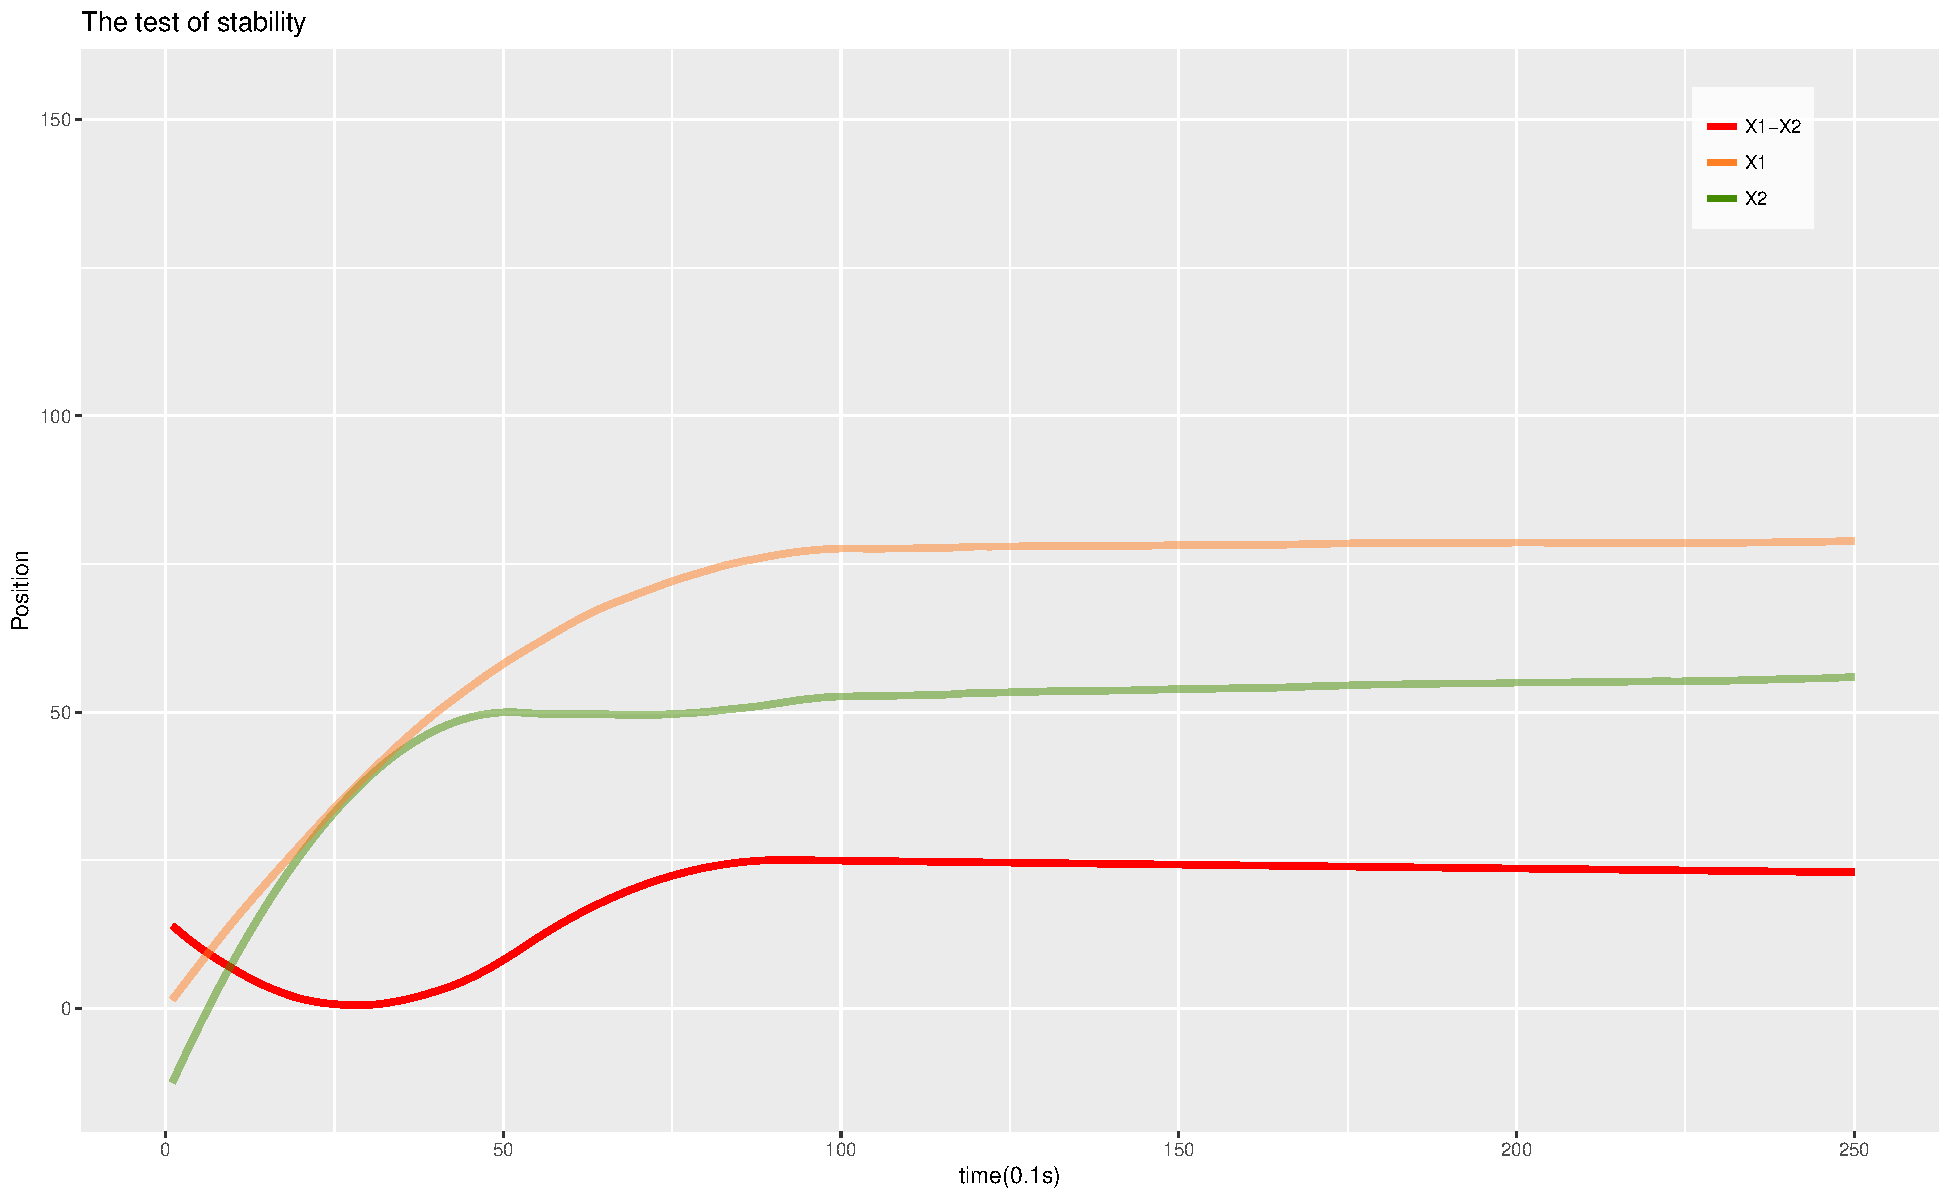
\includegraphics[width=\textwidth]{NearlyGoDie_2.pdf}
\caption{The position of the vehicles and the distance between them}
\label{carf}
\end{figure}

\subsubsection{车路协同驾驶策略}
\label{section:tgs}

除了对车辆的跟驰策略进行了修改,我们也将车辆的自由驾驶模型修正为车路协同的驾驶策略。

为方便后文叙述,我们先定义两个时间参数,最大时间花费$T_{max}$被定义为车辆按照可行的最大加速度$a_{max}$进行减速到最低限速$v_{min}$之后保持匀速直线运动到路口的时间,而最小时间花费$T_{min}$被定义为车辆以最大加速度$a_{max}$进行加速到最高限速$v_{max}$后进行匀速直线运动直到路口所花费的时间。显然,车辆在路中的实际运行时间在$T_{min}$和$T_{max}$之间,并且这两个时间参数之和车辆进入控制路段的初始速度和初始加速度有关。

之后,策略将为车辆在$(T_{min},T_{max}]$区间内为车辆计算定出一个最早的绿灯时间$T_G$。如果上述区间内没有合理的$T_G$绿灯时间,车辆将采取自由驾驶策略。

如果在上述过程中可以定出一个合理的$T_G$,策略将指导车辆按照这个到达时间为目标调整自己的加速度,在这段时间中,如果车辆被前车影响,车辆可能需要重新进入跟驰模型

同时,车辆在交通路口前的表象和之前提到的人工驾驶模型等相同。

总的来说,这个策略是车辆跟驰模型版本的优化版,同时考虑了信号灯相位对于整个路段车辆的影响。

\subsection{多车车路协同模型}
\label{section:st2}
这是一个简单的有车间通信的车路协同主动控制策略。整个策略中队列$Q_{in}$的第一辆车进行处理直到队列的$Q_{in}$的最后一辆车。

首先,对于队列中的$Q_{in}$中的第一辆车,策略使用\ref{section:tgs}中的方法确定一个合适的到达时间$T_G$,为了方便后文表述,我们设定队列$Q_{in}$中的第$n$辆车辆的合理到达时间$T_G$是$T_G^{[n]}$,例如,第一辆车的到达时间就是$T_G^{[1]}$。

在上面确定了$T_G^{[1]}$之后,第一辆车辆将按照设定的合理到达时间$T_G^{[1]}$进行加速或者减速。如果$T_G^{[1]}$不存在,车辆将首先加速到期望速度$v_{exp}$,之后减速到停车线刹车。

之后,我们假定队列$Q_{in}$中的第$n+1$辆车辆能够获得队列$Q_{in}$中的第$n$辆车的合理到达时间$T_G^{[n]}$,包括其是否存在。

The [n+1]-th vehicle determins its $T_G^{[n+1]}$according to its $T_{min}$ and $T_{max}$ and make sure that the $T_G^{[n+1]}-T_G^{[n]} \ge 1 \mathrm{second}$, owing to the fact that the following vehicle is supposed to arrive later than the preceding vehicle.

If the $T_G^{[n]}$ does not exist, $T_G^{[n]+1}$ should be set freely, only depends on the $T_{max}$ and the $T_{min}$ of the vehicle.

Then the acceleration of the [n+1]-th vehicle is set according to the expected time of arrival. The strategy then goes for the following vehicles.

Since the expected time of arrival is carefully designed to make sure that the following vehicle always arrives the stopping line later than the preceding vehicle, even the vehicles which do not have an expected arrival time will take an acceleration, the probability of the rear-ending is minor, a rear-ending will be solve by some simple emergency settings. 

\subsection{The processing of the strategies and the combination of the strategies}
\subsubsection{Single strategy simulation}
The plantform treats the strategies as an iteration from the last vehicle in the $Q_{in}$ to the first one in that, for the reason that the following vehicles may acquire the acceleration of the preceding car which should be fixed until the acceleration is set according to the strategy chosen by user. 

Therefore, if only a specific strategy is chosen, the program behaves like a loop from the last to the first of $Q_{in}$.

\subsubsection{Combination of the strategies}
Only the combination of the manual driving vehicle and the speed guidance models are concerned about, therefore, the plantform only include two kinds of combination simulation, which is the combination between the manual driving vehicle(mentioned in \ref{section:man}) and the single-vehicle cooperative speed guidance model (mentioned in \ref{section:st1}); and the combination between the manual driving vehicle and the multi-vehicle cooperative speed guidence model (mentioned in \ref{section:st2})

During the vehicle generating step, the control strategy of the vehicle is set by random method according to the type of combination and the ratio set by user.

After generate the type of the control strategy, the user-strategy step of the simulation set the acceleration of the vehicle using the strategy it has. It is assmued that if a vehicle using multi-vehicle cooperative speed guidence model is following a manual driving vehicle, the expected arrival time of the manual driving vehicle $T_G$ does not exist, therefore, the speed guidence model could set its expected arrival time $T_G$ freely.

\end{document}